\section{Benchmark producent-klient}

\subsection{Wyniki benchmarków - platforma ARM64}

\begin{figure}[H]
    \centering
    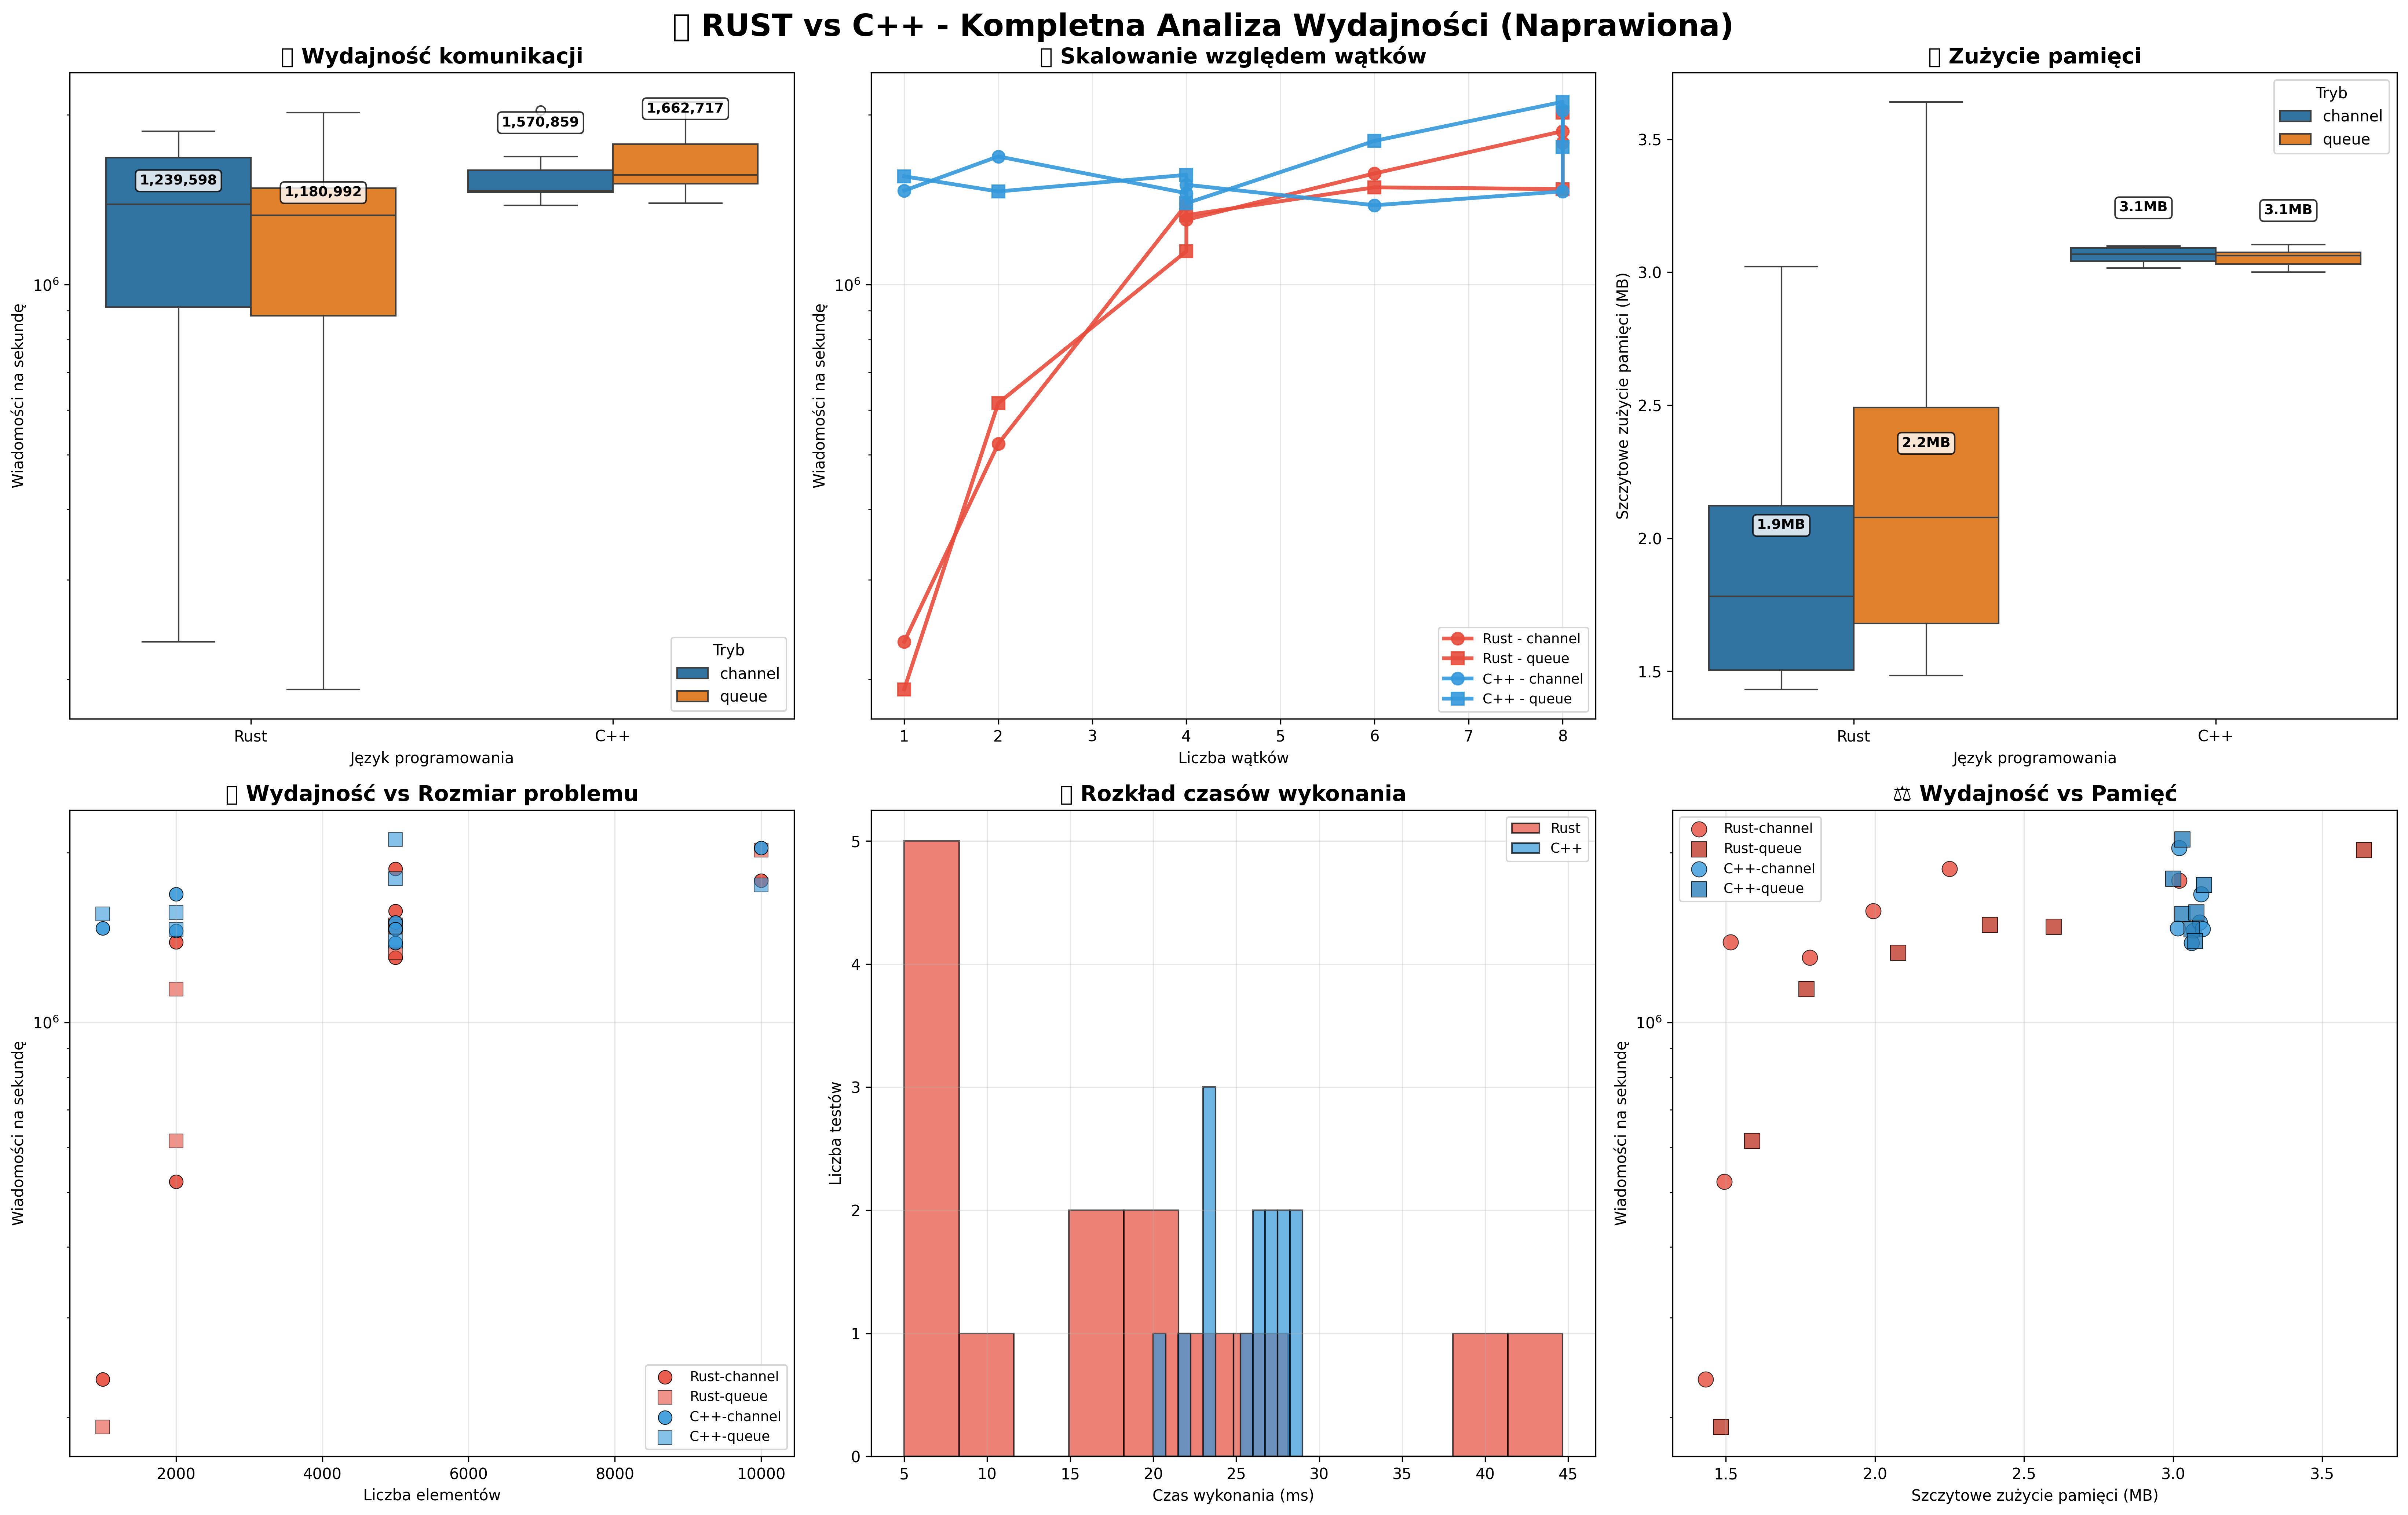
\includegraphics[width=\textwidth]{analiza/images/conc/pc/arm/mega_overview_2x3.png}
    \caption{Analiza wyników benchmarku producent-klient}
    \label{analiza_benchmarku_producent_klient}
\end{figure}

\subsubsection{Wydajność komunikacji międzywątkowej}
Wykres w lewym górnym rogu - rysunek\ref{analiza_benchmarku_producent_klient} przedstawia porównanie przepustowości mechanizmów komunikacji międzywątkowej, wyrażonej liczbą przetworzonych wiadomości na sekundę, dla implementacji w językach Rust i C++. Z analizy wykresów pudełkowych (ang. box plots) wynika, że implementacje w języku C++ charakteryzują się wyższą medianą wydajności w porównaniu do rozwiązań w języku Rust.

Dla implementacji wykorzystującej mechanizm kanału (oznaczony kolorem niebieskim) mediana przepustowości w języku C++ wynosi około 1 570 859 wiadomości na sekundę, podczas gdy analogiczna implementacja w języku Rust osiąga 1 239 598 wiadomości na sekundę, co oznacza przewagę C++ o około 27\%. Podobną zależność obserwujemy dla mechanizmu kolejki (oznaczonego kolorem pomarańczowym), gdzie C++ osiąga 1 662 717 wiadomości na sekundę wobec 1 180 992 dla języka Rust, co daje przewagę wynoszącą około 41\%.

Warto zauważyć, że w przypadku języka C++ implementacja kolejki wykazuje wyższą wydajność niż implementacja kanału, natomiast w języku Rust zależność jest odwrotna. Może to wskazywać na różnice w optymalizacji tych mechanizmów w obu językach.

\subsubsection{Skalowanie względem liczby wątków}
Środkowy górny wykres - rysunek\ref{analiza_benchmarku_producent_klient} ilustruje zależność wydajności od liczby wykorzystywanych wątków. Implementacje w językach Rust i C++ charakteryzują się diametralnie odmiennym wzorcem skalowania. Implementacje C++ (oznaczone kolorem niebieskim) utrzymują względnie stabilną wydajność niezależnie od liczby wątków, z niewielką tendencją wzrostową dla 7-8 wątków w przypadku mechanizmu kolejki.

Natomiast implementacje w języku Rust (oznaczone kolorem czerwonym) rozpoczynają od znacząco niższej wydajności przy 1-2 wątkach, ale wykazują gwałtowny wzrost przepustowości przy zwiększaniu liczby wątków do 4, osiągając wartości zbliżone do implementacji w C++. Ta charakterystyka skalowania sugeruje, że implementacje w języku Rust są zoptymalizowane pod kątem efektywnego wykorzystania równoległości, podczas gdy implementacje w C++ oferują bardziej przewidywalną wydajność niezależną od stopnia paralelizmu.

\subsubsection{Zużycie pamięci}
Prawy górny wykres - rysunek\ref{analiza_benchmarku_producent_klient} przedstawia porównanie zużycia pamięci, mierzonego w megabajtach, dla badanych implementacji. W tym aspekcie język Rust wykazuje wyraźną przewagę, osiągając niższe mediany zużycia pamięci zarówno dla mechanizmu kanału (1,9 MB wobec 3,1 MB w C++), jak i mechanizmu kolejki (2,2 MB wobec 3,1 MB w C++).

Ta różnica, wynosząca około 40\% dla mechanizmu kanału i 29\% dla mechanizmu kolejki, może być przypisana efektywnemu systemowi zarządzania pamięcią w języku Rust, bazującemu na analizie czasu życia (ang. lifetime analysis) i systemie własności (ang. ownership system), które eliminują konieczność stosowania kosztownych mechanizmów automatycznego odzyskiwania pamięci (ang. garbage collection) lub podatność na wycieki pamięci charakterystyczne dla ręcznego zarządzania pamięcią w C++.

\subsubsection{ Rozkład czasów wykonania}
Środkowy dolny histogram - rysunek\ref{analiza_benchmarku_producent_klient} prezentuje rozkład częstości czasów wykonania dla implementacji w językach Rust (kolor czerwony) i C++ (kolor niebieski). Analiza tego wykresu ujawnia fundamentalne różnice w charakterystykach wydajnościowych obu języków.

Implementacje w języku Rust charakteryzują się bimodalnym rozkładem czasów wykonania, z dominującym szczytem przy około 5 ms oraz mniejszymi skupiskami w okolicach 15-20 ms i 40-45 ms. Taka dystrybucja może świadczyć o różnych strategiach optymalizacji w zależności od specyfiki zadania lub wpływie dodatkowych mechanizmów zarządzania pamięcią.

W przeciwieństwie do tego, czasy wykonania dla implementacji C++ koncentrują się głównie w przedziale 20-25 ms, z mniejszą wariancją, co wskazuje na bardziej przewidywalną wydajność, potencjalnie kosztem utraconych możliwości optymalizacji w określonych scenariuszach.

\subsubsection{Wydajność względem zużycia pamięci}
Prawy dolny wykres - rysunek\ref{analiza_benchmarku_producent_klient} przedstawia relację między wydajnością a szczytowym zużyciem pamięci. Punkty danych tworzą wyraźnie odrębne skupiska dla implementacji w języku Rust (punkty czerwone) i C++ (punkty niebieskie). Implementacje C++ charakteryzują się wyższą wydajnością przy jednoczesnym wyższym zużyciu pamięci, koncentrując się w górnym prawym obszarze wykresu.

Z kolei implementacje w języku Rust wykazują większe rozproszenie, zarówno pod względem wydajności, jak i zużycia pamięci, co sugeruje większą adaptacyjność tych implementacji do różnych warunków wykonania. Szczególnie interesujące są pojedyncze punkty dla implementacji Rust o bardzo niskim zużyciu pamięci (około 1,5 MB) i jednocześnie niskiej wydajności, które mogą reprezentować skrajne przypadki optymalizacji pod kątem oszczędności zasobów kosztem wydajności.

\subsubsection{Podsumowanie}
Przeprowadzona analiza porównawcza mechanizmów współbieżności w językach Rust i C++ ujawnia istotne kompromisy wydajnościowe. Implementacje C++ oferują generalnie wyższą przepustowość, szczególnie przy mniejszej liczbie wątków i mniejszych rozmiarach problemu, jednak kosztem zwiększonego zużycia pamięci. Z kolei implementacje w języku Rust charakteryzują się niższym zużyciem zasobów pamięciowych oraz znakomitym skalowaniem wydajności wraz ze wzrostem stopnia równoległości, choć przy niskim poziomie paralelizmu ustępują wydajnością rozwiązaniom w C++.

Wyniki badań sugerują, że wybór między tymi językami powinien być podyktowany specyfiką zastosowania: w systemach o ograniczonych zasobach pamięciowych lub wymagających wysokiej skalowalności Rust może oferować lepsze rozwiązania, natomiast w zastosowaniach priorytetyzujących maksymalną przepustowość przy niewielkiej liczbie wątków lub przewidywalność czasów wykonania implementacje C++ mogą stanowić bardziej odpowiedni wybór.

Warto również zauważyć, że w obu językach mechanizm kolejki wykazuje odmienne charakterystyki wydajnościowe w porównaniu do mechanizmu kanału, co dodatkowo podkreśla złożoność decyzji projektowych w kontekście programowania współbieżnego.
\subsection{Wyniki benchmarków - platforma x86\_64}
\begin{figure}[H]
    \centering
    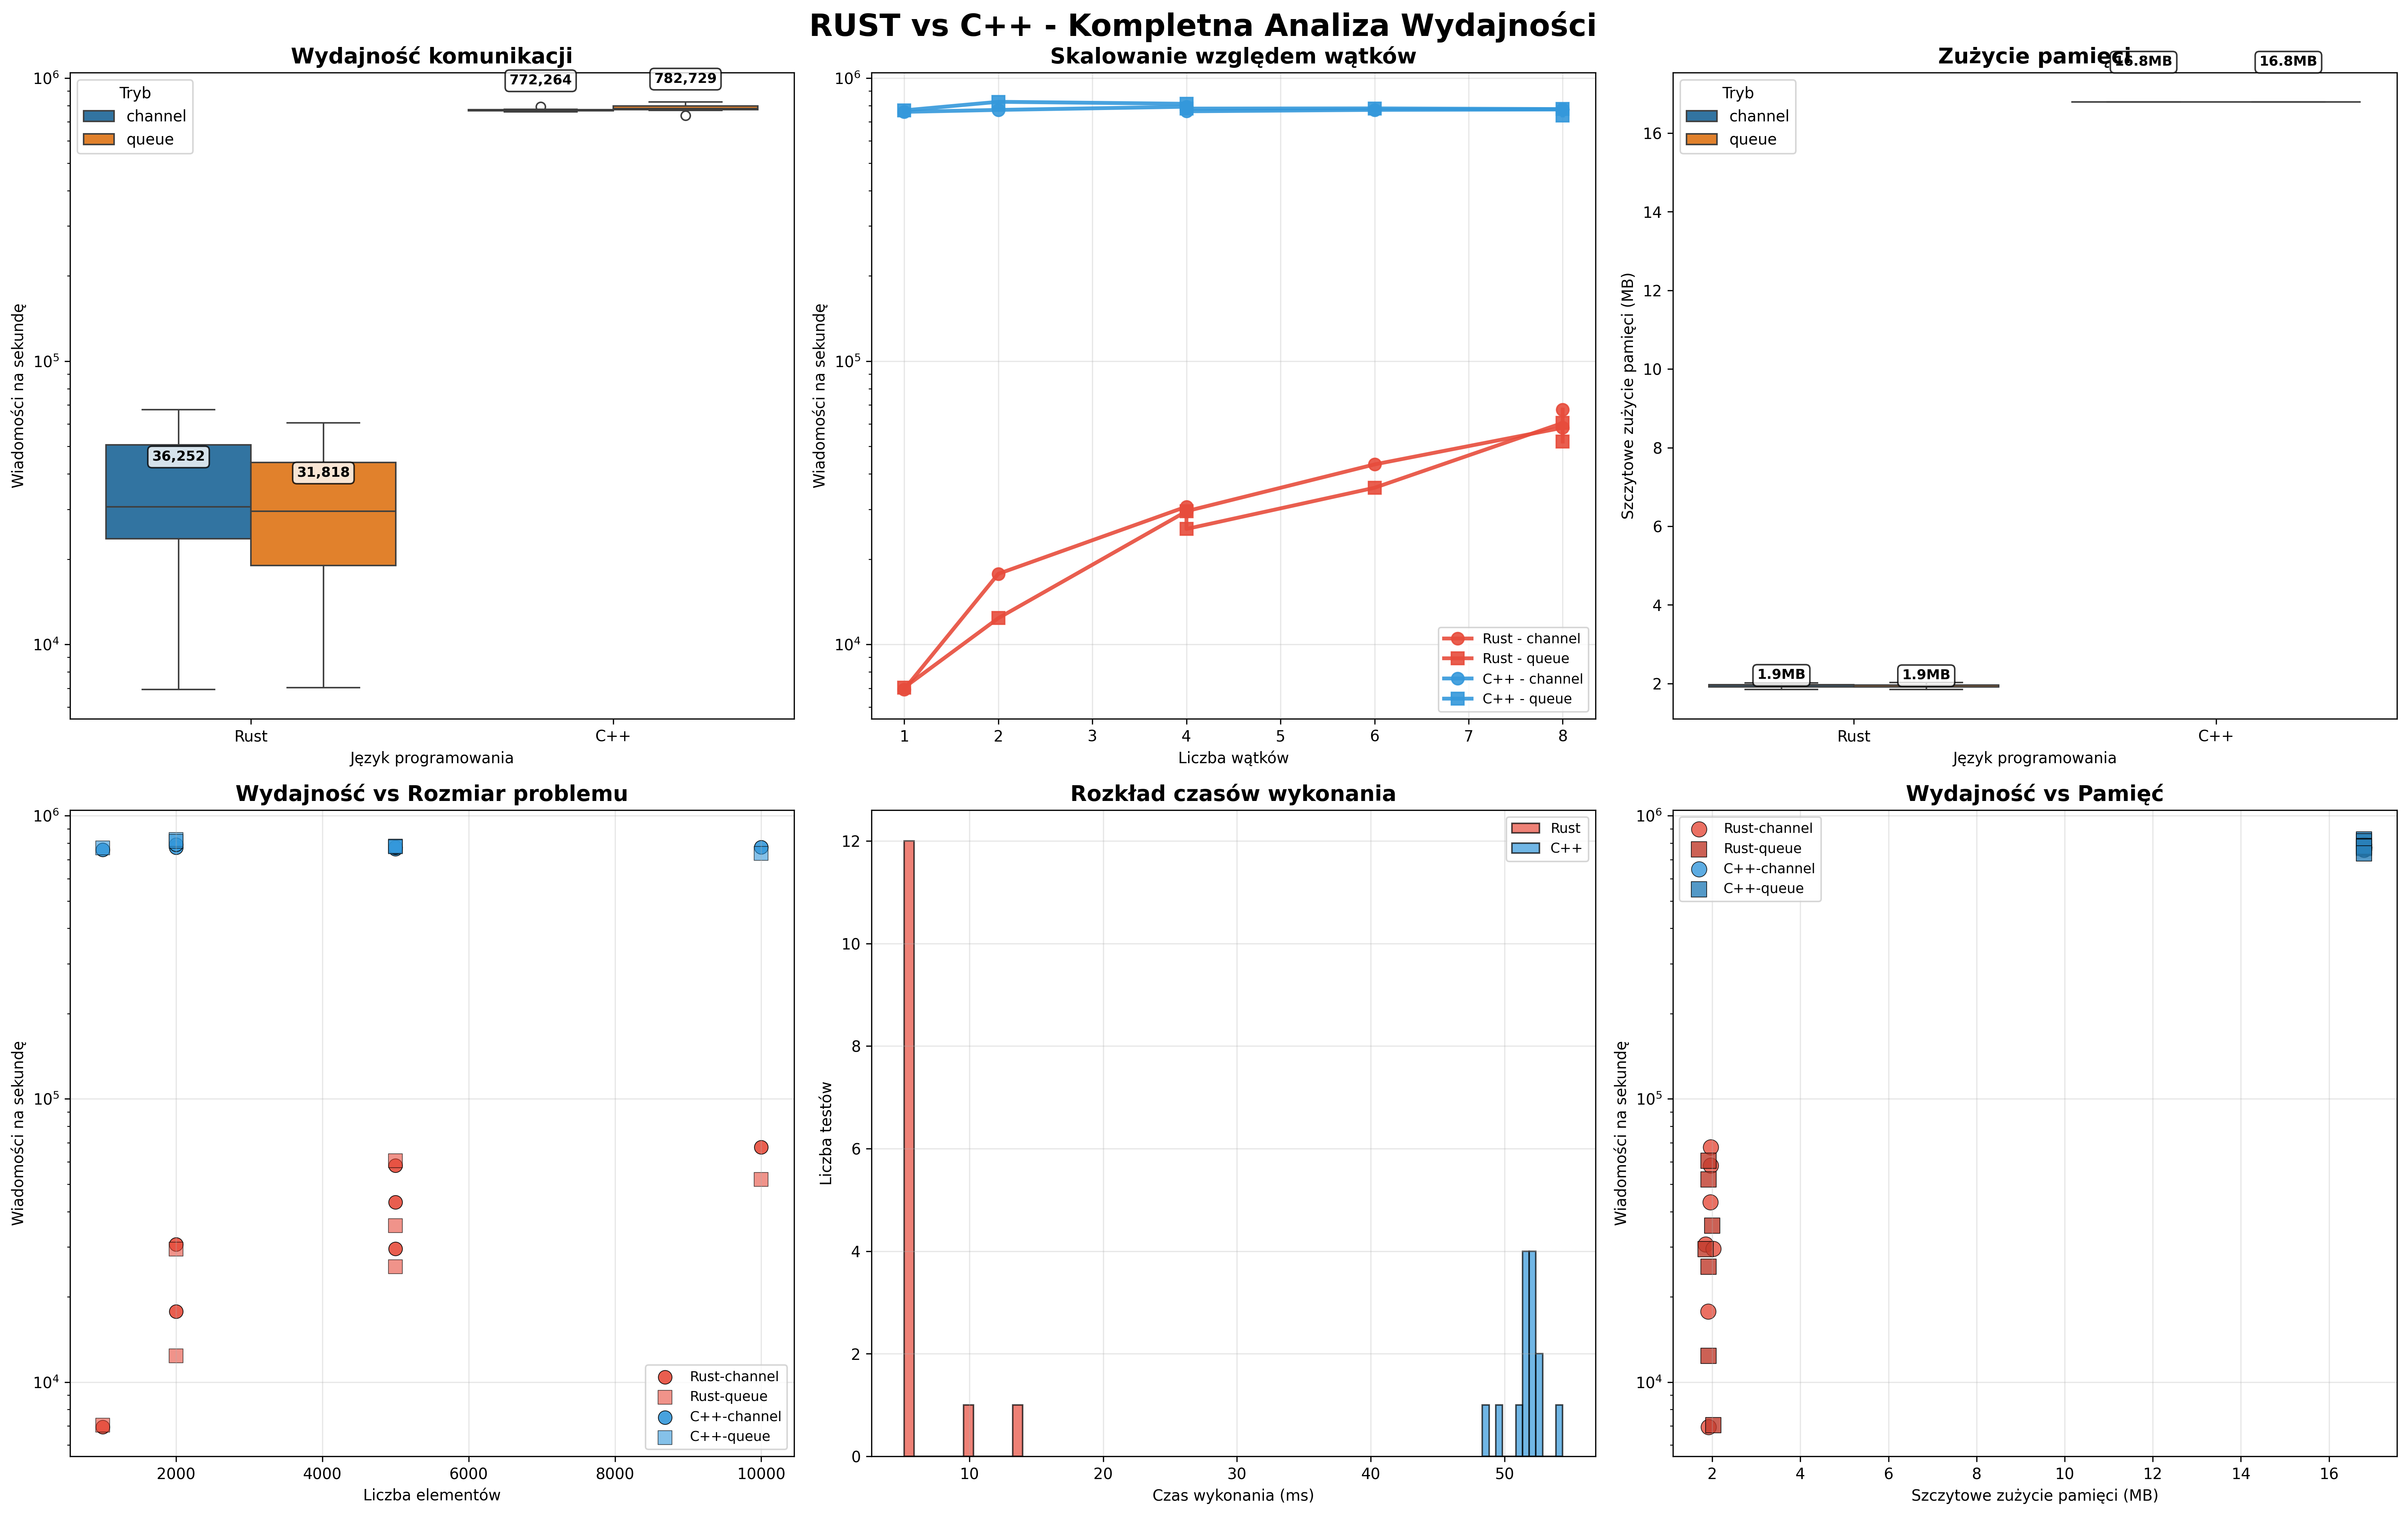
\includegraphics[width=\textwidth]{analiza/images/conc/pc/x86/mega_overview_2x3.png}
    \caption{Analiza wyników benchmarku producent-klient}
    \label{analiza_benchmarku_producent_klient_x86_64}
\end{figure}

\subsubsection{Wydajność komunikacji międzywątkowej}
Wykres w lewym górnym rogu - rysunek \ref{analiza_benchmarku_producent_klient_x86_64} przedstawia porównanie przepustowości mechanizmów komunikacji międzywątkowej, wyrażonej liczbą wiadomości przetwarzanych na sekundę. Analiza wykresu pudełkowego (ang. box plot) wskazuje na znaczącą różnicę wydajności między implementacjami w językach C++ i Rust.

Implementacje w języku C++ osiągają znacząco wyższą przepustowość, z medianą na poziomie 772 264 wiadomości/s dla mechanizmu kanału (kolor niebieski) i 782 729 wiadomości/s dla mechanizmu kolejki (kolor pomarańczowy). W przeciwieństwie do tego, implementacje w języku Rust osiągają przepustowość rzędu 36 252 wiadomości/s dla mechanizmu kanału i 31 818 wiadomości/s dla mechanizmu kolejki.

Ta dysproporcja, wyrażająca się współczynnikiem około 21:1 na korzyść C++, wskazuje na fundamentalne różnice w wydajności bazowych mechanizmów komunikacji międzywątkowej w obu językach. Warto zauważyć, że rozrzut wartości (wysokość prostokątów) jest znacznie większy w przypadku implementacji Rust, co sugeruje mniej przewidywalną wydajność w porównaniu do bardziej stabilnych wyników w C++.

\subsubsection{Skalowanie względem liczby wątków}
Środkowy górny wykres - rysunek \ref{analiza_benchmarku_producent_klient_x86_64} ilustruje zależność pomiędzy liczbą wykorzystywanych wątków a osiąganą przepustowością komunikacji. Różnice w charakterystyce skalowania między językami są uderzające. Implementacje w języku C++ (niebieskie linie) utrzymują stałą, wysoką wydajność na poziomie około $10^5$ wiadomości/s, praktycznie niezależnie od liczby wykorzystywanych wątków.

W przeciwieństwie do tego, implementacje w języku Rust (czerwone linie) wykazują wyraźną zależność od liczby wątków. Rozpoczynając od wydajności rzędu $6\times10^3$ wiadomości/s przy jednym wątku, osiągają około $7\times10^4$ wiadomości/s przy ośmiu wątkach, co stanowi ponad dziesięciokrotną poprawę. Pomimo tego znaczącego wzrostu wydajności, nawet przy maksymalnej liczbie wątków implementacje Rust nie osiągają poziomu wydajności oferowanego przez C++.

Taka charakterystyka może wskazywać na odmienne podejścia do optymalizacji w obu językach: C++ może być zoptymalizowany pod kątem maksymalnej przepustowości pojedynczego wątku, podczas gdy Rust może priorytetyzować efektywne wykorzystanie wielu rdzeni kosztem wydajności pojedynczego wątku.


\subsubsection{Zużycie pamięci}
Prawy górny wykres - rysunek \ref{analiza_benchmarku_producent_klient_x86_64} przedstawia porównanie zużycia pamięci dla analizowanych implementacji. W przeciwieństwie do wyników wydajnościowych, to język Rust wykazuje zdecydowaną przewagę pod względem efektywności wykorzystania zasobów pamięciowych. Zarówno implementacja wykorzystująca kanał, jak i implementacja wykorzystująca kolejkę w języku Rust wykazują zużycie pamięci na poziomie 1,9 MB.

Dla porównania, obie implementacje w języku C++ charakteryzują się zużyciem pamięci na poziomie 16,8 MB, co stanowi prawie dziewięciokrotnie wyższe zapotrzebowanie na pamięć w porównaniu do rozwiązań w Rust. Ta różnica wynika prawdopodobnie z odmiennych podejść do zarządzania pamięcią: Rust wykorzystuje system własności (ang. ownership system) i analizę czasu życia obiektów (ang. lifetime analysis), co pozwala na bardziej efektywne zarządzanie zasobami pamięciowymi.

\subsubsection{Wydajność względem rozmiaru problemu}
Lewy dolny wykres - rysunek \ref{analiza_benchmarku_producent_klient_x86_64} ilustruje zależność wydajności od rozmiaru problemu, wyrażonego liczbą przetwarzanych elementów. Ponownie obserwujemy wyraźną przewagę wydajnościową implementacji C++ (niebieskie punkty) nad implementacjami Rust (czerwone punkty) w całym spektrum badanych rozmiarów problemu.

Implementacje C++ utrzymują stałą, wysoką wydajność rzędu $10^5$ wiadomości/s niezależnie od rozmiaru problemu. Implementacje Rust wykazują ogólnie niższą wydajność rzędu $10^1$ do $10^2$ wiadomości/s, z nieznaczną tendencją wzrostową wraz ze zwiększaniem rozmiaru problemu, szczególnie widoczną przy przejściu z 2000 do 6000 elementów. Może to sugerować, że koszty inicjalizacji i zarządzania w Rust są amortyzowane przy większych rozmiarach problemu.



\subsubsection{Rozkład czasów wykonania}
Środkowy dolny histogram - rysunek \ref{analiza_benchmarku_producent_klient_x86_64} prezentuje rozkład czasów wykonania dla implementacji w językach Rust (kolor czerwony) i C++ (kolor niebieski). Zaskakujące jest to, że mimo niższej przepustowości komunikacji, implementacje w języku Rust charakteryzują się znacznie krótszymi czasami wykonania, z dominującym skupiskiem w okolicach 5-10 ms.

W przeciwieństwie do tego, czasy wykonania dla implementacji C++ koncentrują się w przedziale 50-55 ms. Ta pozorna sprzeczność między krótszymi czasami wykonania a niższą przepustowością komunikacji w języku Rust może wskazywać na różnice w metodologii pomiaru lub na wyższe narzuty związane z inicjalizacją komunikacji w Rust, które nie są uwzględniane w bezpośrednim pomiarze czasu wykonania.

\subsubsection{Wydajność względem zużycia pamięci}
Prawy dolny wykres - rysunek \ref{analiza_benchmarku_producent_klient_x86_64} przedstawia relację między wydajnością a zużyciem pamięci. Punkty danych tworzą wyraźnie odrębne skupiska dla implementacji w języku Rust (czerwone punkty) i C++ (niebieskie punkty). Implementacje C++ charakteryzują się wysoką wydajnością (około $10^5$ wiadomości/s) przy wysokim zużyciu pamięci (16 MB), podczas gdy implementacje Rust oferują niższą wydajność ($10^1$ do $10^2$ wiadomości/s) przy znacznie niższym zużyciu pamięci (około 2 MB).

Ta dystrybucja punktów ilustruje fundamentalny kompromis między wydajnością a efektywnością wykorzystania zasobów, który jest kluczowym czynnikiem przy wyborze odpowiedniej technologii dla konkretnych zastosowań. Warto zauważyć, że implementacje w tym samym języku tworzą zwarte skupiska, co sugeruje, że różnice między mechanizmem kanału a kolejki są mniej istotne niż różnice wynikające z wyboru języka programowania.

\subsubsection{Podsumowanie}
Przeprowadzona analiza porównawcza mechanizmów współbieżności w językach Rust i C++ ujawnia fundamentalnie odmienne charakterystyki wydajnościowe. Implementacje w języku C++ oferują znacząco wyższą przepustowość komunikacji międzywątkowej, która utrzymuje się na stabilnym poziomie niezależnie od liczby wątków czy rozmiaru problemu. Z kolei implementacje w języku Rust, mimo niższej bezwzględnej przepustowości, charakteryzują się znacznie niższym zużyciem pamięci oraz lepszymi właściwościami skalowania wraz ze wzrostem liczby wątków.

Szczególnie interesująca jest obserwacja, że pomimo niższej przepustowości, implementacje Rust osiągają krótsze czasy wykonania, co może wskazywać na niższe opóźnienia w przetwarzaniu pojedynczych operacji, nawet jeśli łączna liczba operacji na sekundę jest niższa niż w przypadku C++.

\subsection{Porównanie pomiędzy platformami}
\begin{figure}[H]
    \centering
    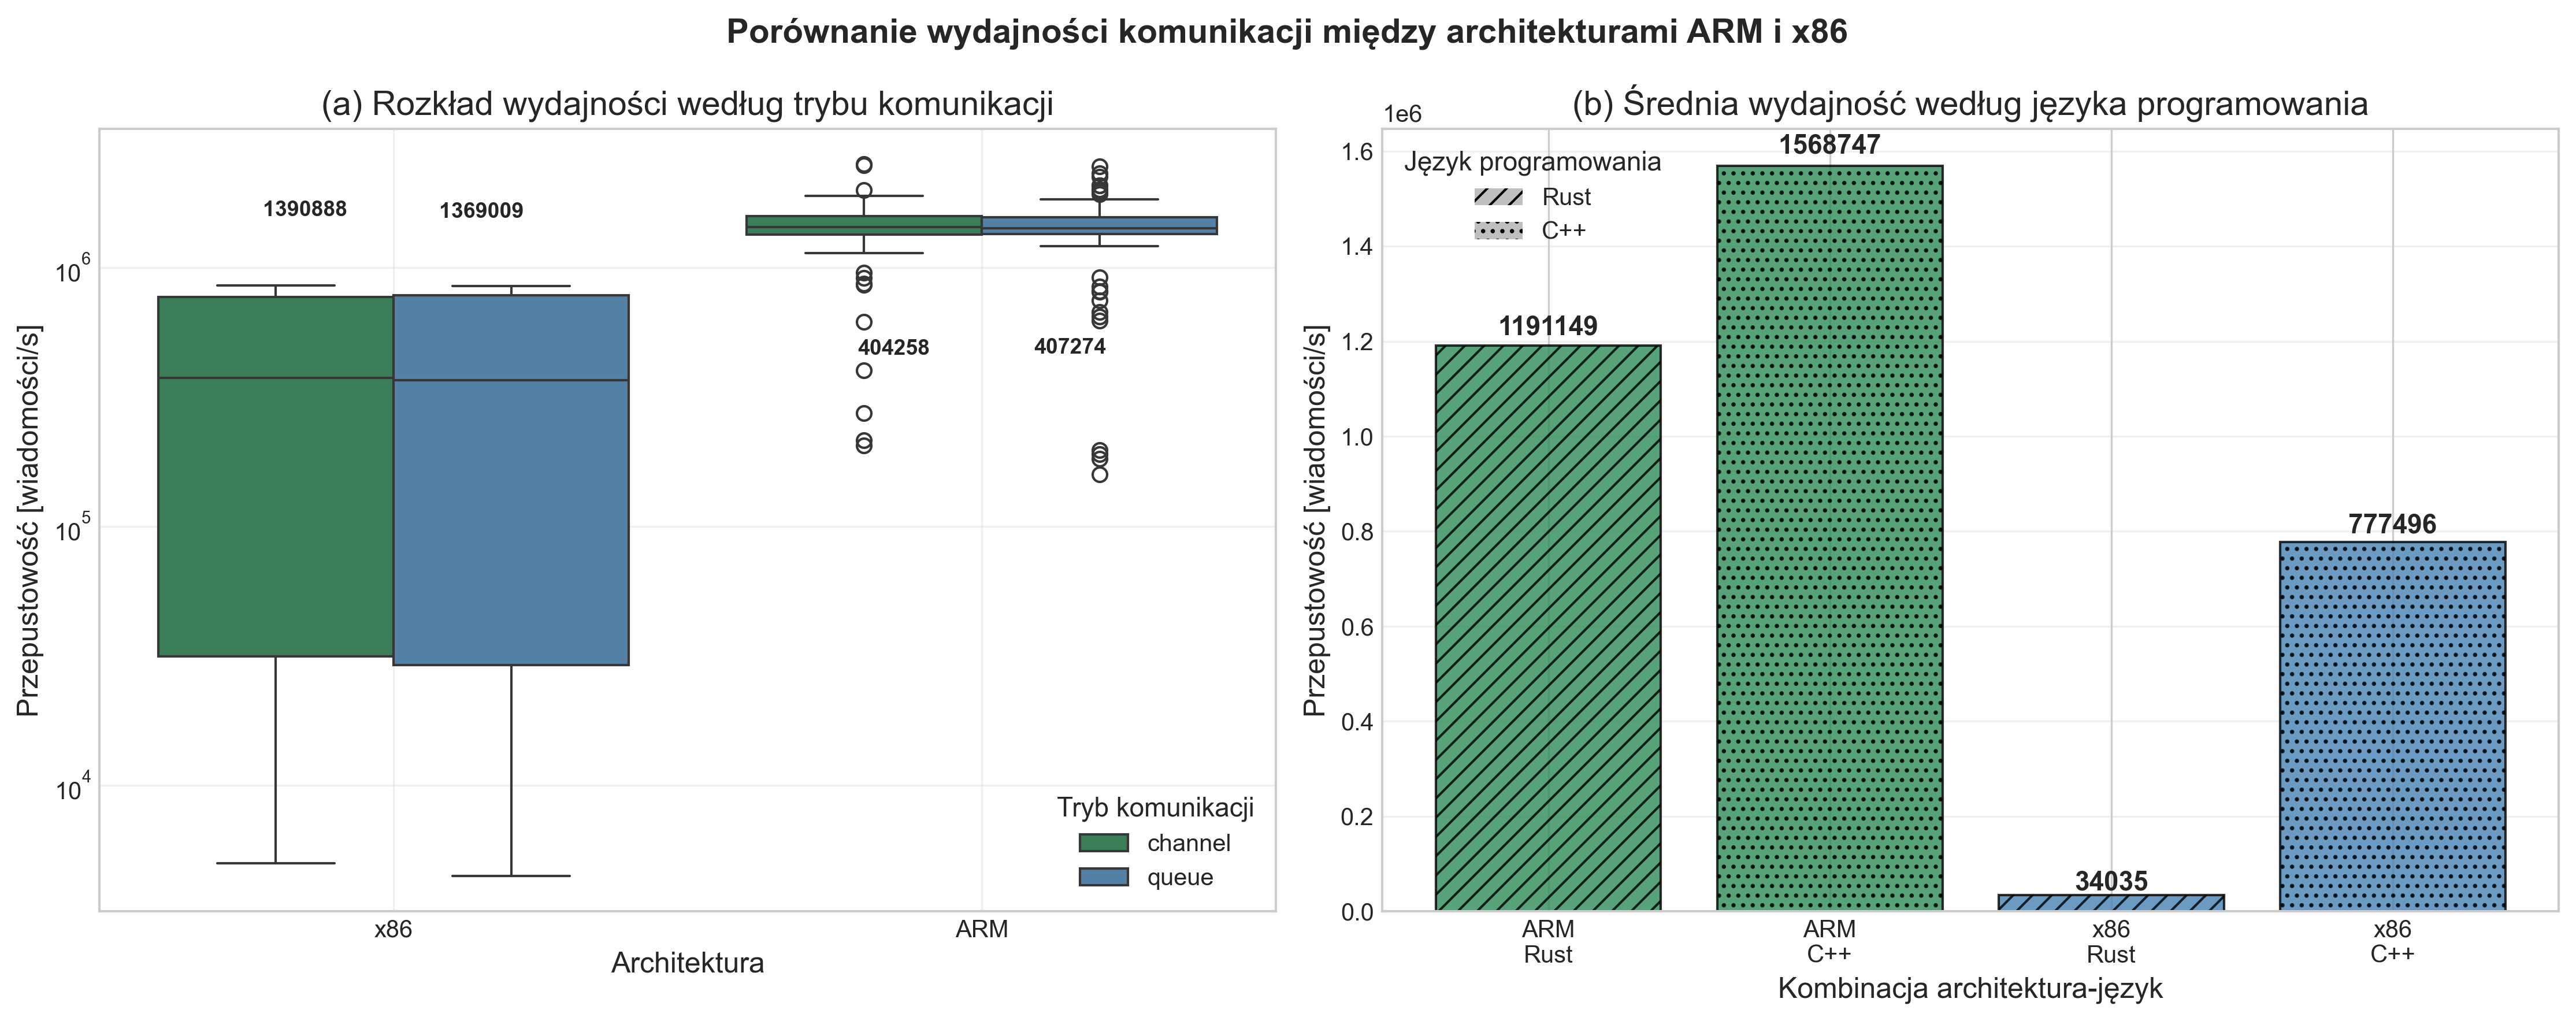
\includegraphics[width=\textwidth]{analiza/images/conc/pc/compare/rysunek_1_porownanie_wydajnosci.png}
    \caption{Porównanie wydajności komunikacji między architekturami ARM i x86}
    \label{rysunek_1_porownanie_wydajnosci}
\end{figure}
\subsubsection{Rozkład wydajności według trybu komunikacji}
Na wykresie (a) - rysunek \ref{rysunek_1_porownanie_wydajnosci} przedstawiono porównanie przepustowości mechanizmów komunikacji międzywątkowej dla architektur x86 i ARM, z rozróżnieniem na mechanizm kanału (kolor zielony) i kolejki (kolor niebieski). Analiza danych wskazuje na diametralną różnicę wydajnościową między badanymi architekturami:
\begin{itemize}
    \item W przypadku architektury x86, mechanizmy komunikacji osiągają mediany przepustowości na poziomie 1 390 888 wiadomości/s (kanał) i 1 369 009 wiadomości/s (kolejka).
    \item Dla architektury ARM, wartości te wynoszą odpowiednio 404 258 wiadomości/s (kanał) i 407 274 wiadomości/s (kolejka).
\end{itemize}

Można zaobserwować zatem, że architektura x86 zapewnia około 3,4-krotnie wyższą przepustowość w porównaniu do architektury ARM, niezależnie od zastosowanego mechanizmu komunikacji. Warto zauważyć, że w obrębie tej samej architektury wybór między mechanizmem kanału a kolejki ma marginalne znaczenie dla osiąganej wydajności.

\subsubsection{Średnia wydajność według języka programowania}
Wykres (b) - rysunek \ref{rysunek_1_porownanie_wydajnosci} dostarcza bardziej szczegółowej analizy, uwzględniającej dodatkowy wymiar w postaci języka implementacji. Wyniki wykazują interesującą interakcję między architekturą a językiem programowania:
\begin{itemize}
    \item Najwyższą wydajność osiąga kombinacja ARM + C++ (1 568 747 wiadomości/s), przewyższając znacząco pozostałe konfiguracje.
    \item Na drugim miejscu plasuje się ARM + Rust (1 191 149 wiadomości/s), osiągając 76\% wydajności implementacji C++ na tej samej architekturze.
    \item Implementacja x86 + C++ (777 496 wiadomości/s) osiąga zaledwie 50\% wydajności najlepszej konfiguracji.
    \item Szczególnie niska wydajność cechuje kombinację x86 + Rust (34 035 wiadomości/s), stanowiącą tylko 2,2\% wydajności lidera.
\end{itemize}

\begin{figure}[H]
    \centering
    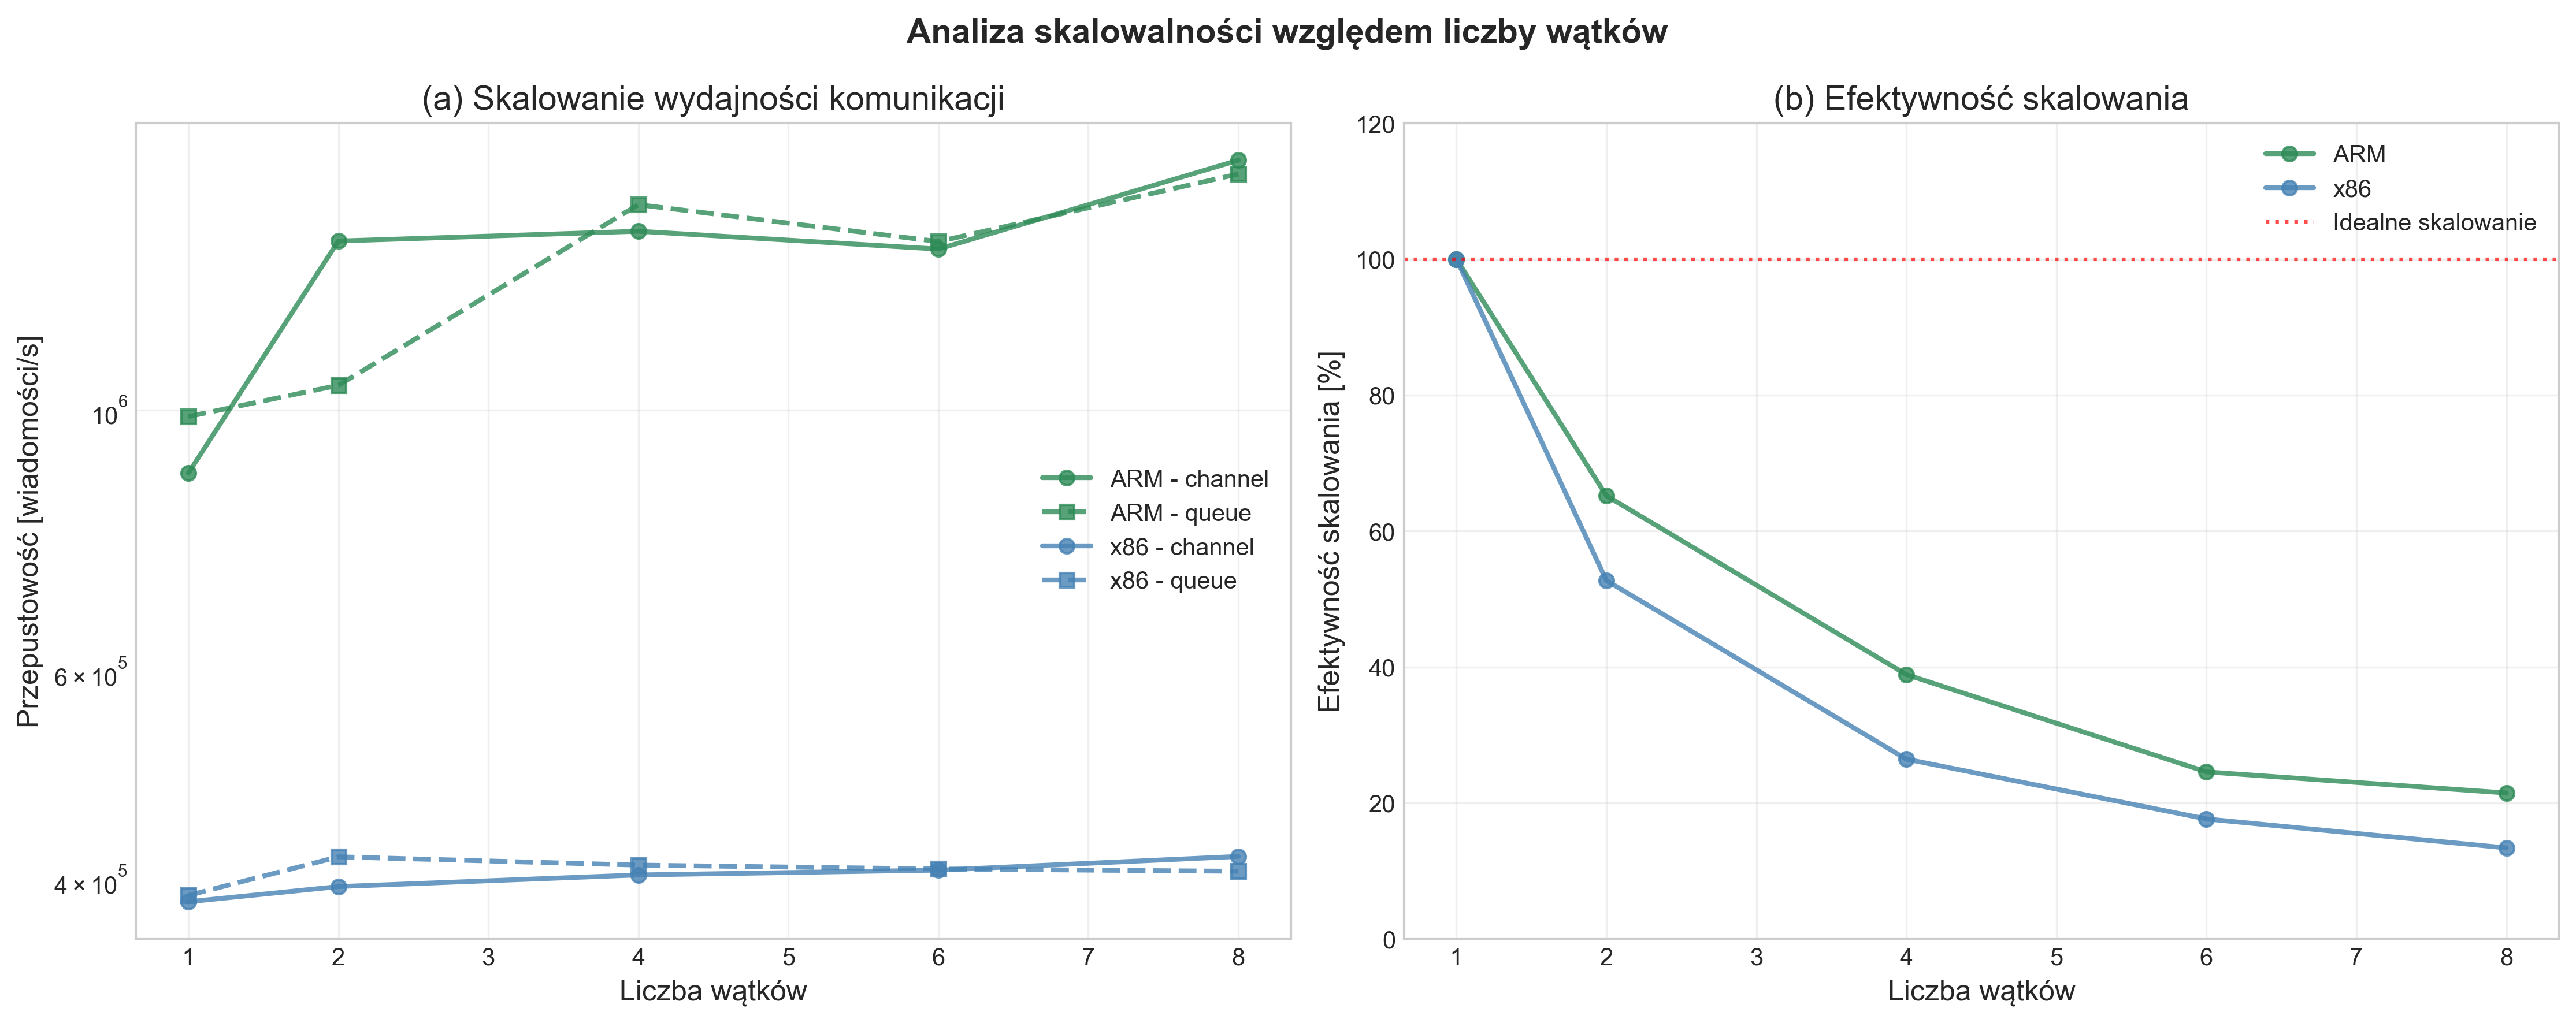
\includegraphics[width=\textwidth]{analiza/images/conc/pc/compare/rysunek_2_skalowanie_watkow.png}
    \caption{Analiza skalowania względem liczby wątków}
    \label{rysunek_2_skalowanie_watkow}
\end{figure}
\subsubsection{Skalowanie wydajności komunikacji}
Wykres (a) - rysunek \ref{rysunek_2_skalowanie_watkow} przedstawia zależność przepustowości komunikacji międzywątkowej od liczby wykorzystywanych wątków dla dwóch architektur sprzętowych: ARM i x86, z dalszym podziałem na implementację z wykorzystaniem mechanizmu kanału (linie ciągłe) i kolejki (linie przerywane).

Analiza danych ujawnia fundamentalne różnice w charakterystyce skalowania obu architektur:
\begin{itemize}
    \item Architektura ARM wykazuje znacząco wyższy potencjał skalowania niż x86, osiągając przepustowość około 1,8 mln wiadomości na sekundę przy 8 wątkach, podczas gdy x86 utrzymuje się na poziomie około 0,4-0,5 mln wiadomości/s niezależnie od liczby wątków.
    \item Implementacje ARM charakteryzują się gwałtownym wzrostem wydajności przy przejściu z 1 do 2 wątków dla mechanizmu kanału (wzrost z około 0,8 mln do 1,7 mln wiadomości/s), podczas gdy mechanizm kolejki wykazuje bardziej stopniowy wzrost, osiągając porównywalną wydajność dopiero przy 4 wątkach.
    \item Obie implementacje na architekturze x86 (zarówno kanał, jak i kolejka) wykazują minimalny wzrost wydajności wraz ze zwiększaniem liczby wątków, co sugeruje istotne ograniczenia skalowania w tej architekturze w kontekście komunikacji międzywątkowej.
\end{itemize}

\subsubsection{Efektywność skalowania}
Wykres (b) - rysunek \ref{rysunek_2_skalowanie_watkow} kwantyfikuje efektywność skalowania dla obu architektur, wyrażoną jako odsetek idealnego skalowania liniowego (zaznaczonego czerwoną przerywaną linią na poziomie 100\%).

Kluczowe obserwacje:
\begin{itemize}
    \item Obie architektury wykazują spadek efektywności skalowania wraz ze wzrostem liczby wątków, co jest zjawiskiem oczekiwanym ze względu na rosnące koszty synchronizacji i współdzielenia zasobów.
    \item Architektura ARM (linia zielona) konsekwentnie utrzymuje wyższą efektywność skalowania niż x86 (linia niebieska) w całym spektrum badanych konfiguracji wątkowych.
    \item Przy 2 wątkach, architektura ARM zachowuje około 65\% efektywności skalowania, podczas gdy x86 - około 53\%. Różnica ta pogłębia się przy większej liczbie wątków.
    \item Przy maksymalnej badanej liczbie 8 wątków, ARM utrzymuje około 21\% efektywności idealnego skalowania, podczas gdy x86 osiąga zaledwie około 13\%.
\end{itemize}

\begin{figure}[H]
    \centering
    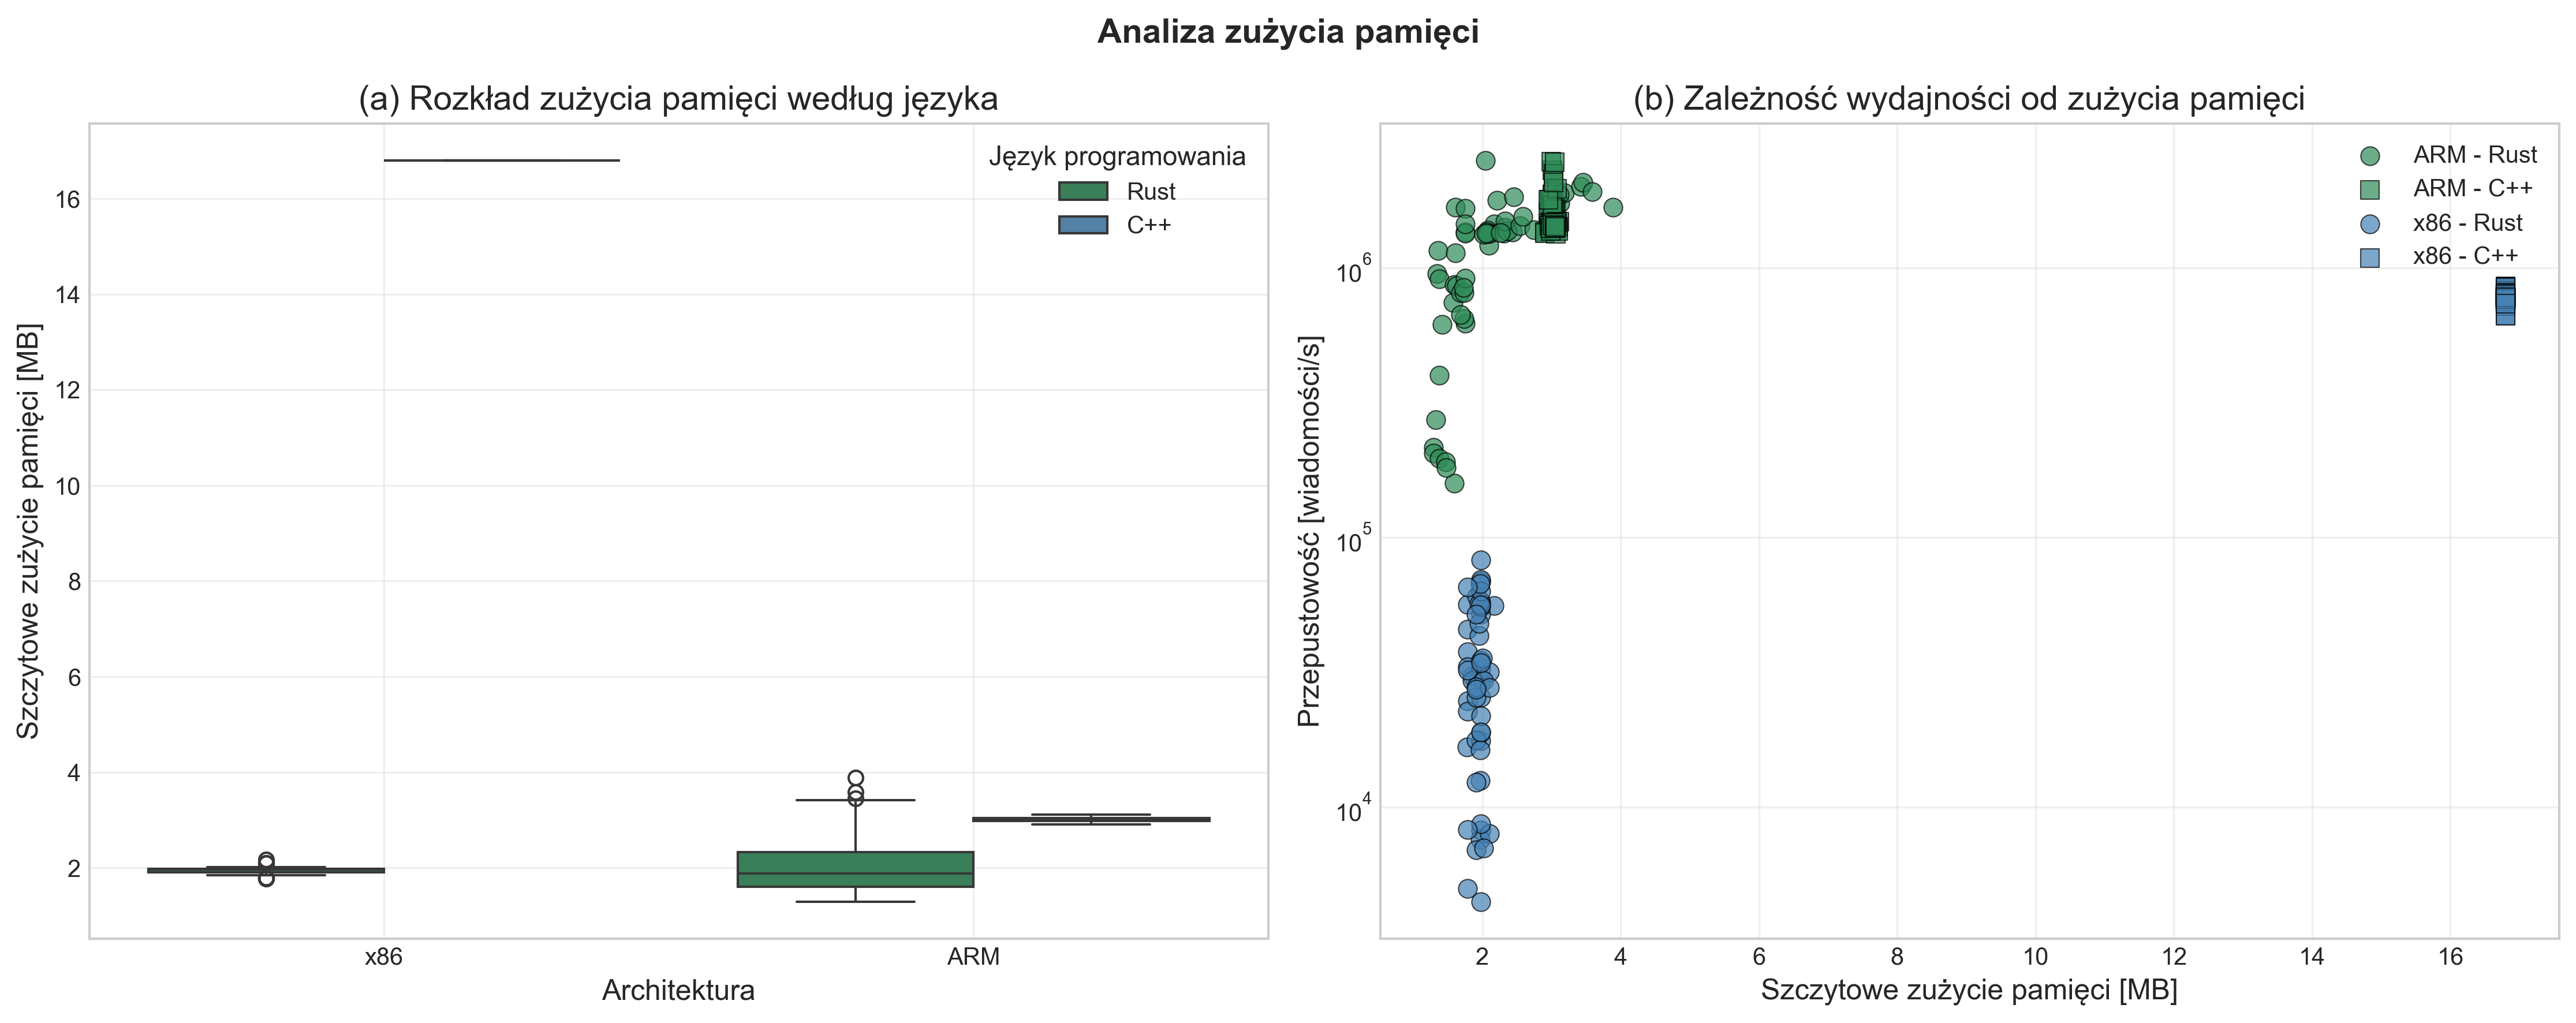
\includegraphics[width=\textwidth]{analiza/images/conc/pc/compare/rysunek_3_zuzycie_pamieci.png}
    \caption{Analiza zużycia pamięci}
    \label{rysunek_3_zuzycie_pamieci}
\end{figure}

\subsubsection{Rozkład zużycia pamięci według języka i architektury}
Wykres (a) - rysunek \ref{rysunek_3_zuzycie_pamieci} przedstawia porównanie szczytowego zużycia pamięci dla implementacji mechanizmów współbieżności w językach Rust (kolor zielony) i C++ (kolor niebieski) na architekturach x86 i ARM. Z analizy danych wynika, że:
\begin{itemize}
    \item Architektura x86 charakteryzuje się mniejszym zużyciem pamięci (mediana około 2 MB) w porównaniu do architektury ARM (mediana około 2,2 MB).
    \item Implementacje na architekturze ARM wykazują większy rozrzut wartości zużycia pamięci, co widoczne jest w szerszym zakresie wykresu pudełkowego oraz obecności wartości odstających sięgających nawet 4 MB.
    \item Różnice między językami programowania w kontekście zużycia pamięci są minimalnie, zarówno na architekturze ARM, jak i x86, co sugeruje, że to głównie architektura sprzętowa, a nie wybór języka programowania, determinuje profil pamięciowy aplikacji współbieżnych.
\end{itemize}

\subsubsection{Zależność wydajności od zużycia pamięci}
Wykres (b) - rysunek \ref{rysunek_3_zuzycie_pamieci} ilustruje relację między szczytowym zużyciem pamięci a osiąganą przepustowością komunikacji dla czterech kombinacji: ARM-Rust (ciemnozielone kółka), ARM-C++ (jasnozielone kwadraty), x86-Rust (jasnoniebieskie kółka) i x86-C++ (ciemnoniebieskie kwadraty). Analiza tego wykresu ujawnia kilka istotnych zależności:
\begin{itemize}
    \item Implementacje na architekturze ARM osiągają znacząco wyższą przepustowość (rzędu $10^6$ wiadomości/s) w porównaniu do implementacji na architekturze x86 (rzędu $10^4$-$10^5$ wiadomości/s), przy tylko nieznacznie wyższym zużyciu pamięci.
    \item Punkty danych dla architektury ARM tworzą zwartą grupę w prawym górnym obszarze wykresu, co sugeruje stabilną wydajność przy podobnym zużyciu pamięci niezależnie od wybranego języka programowania.
    \item Implementacje na architekturze x86 charakteryzują się większym rozproszeniem punktów wzdłuż osi zużycia pamięci, szczególnie widocznym dla języka C++, gdzie obserwujemy punkty od około 2 MB do nawet 16 MB.
    \item Najbardziej efektywną kombinacją pod względem stosunku wydajności do zużycia pamięci wydają się być implementacje ARM-Rust, które osiągają wysoką przepustowość przy relatywnie niskim i stabilnym zużyciu pamięci.
\end{itemize}



\begin{figure}[H]
    \centering
    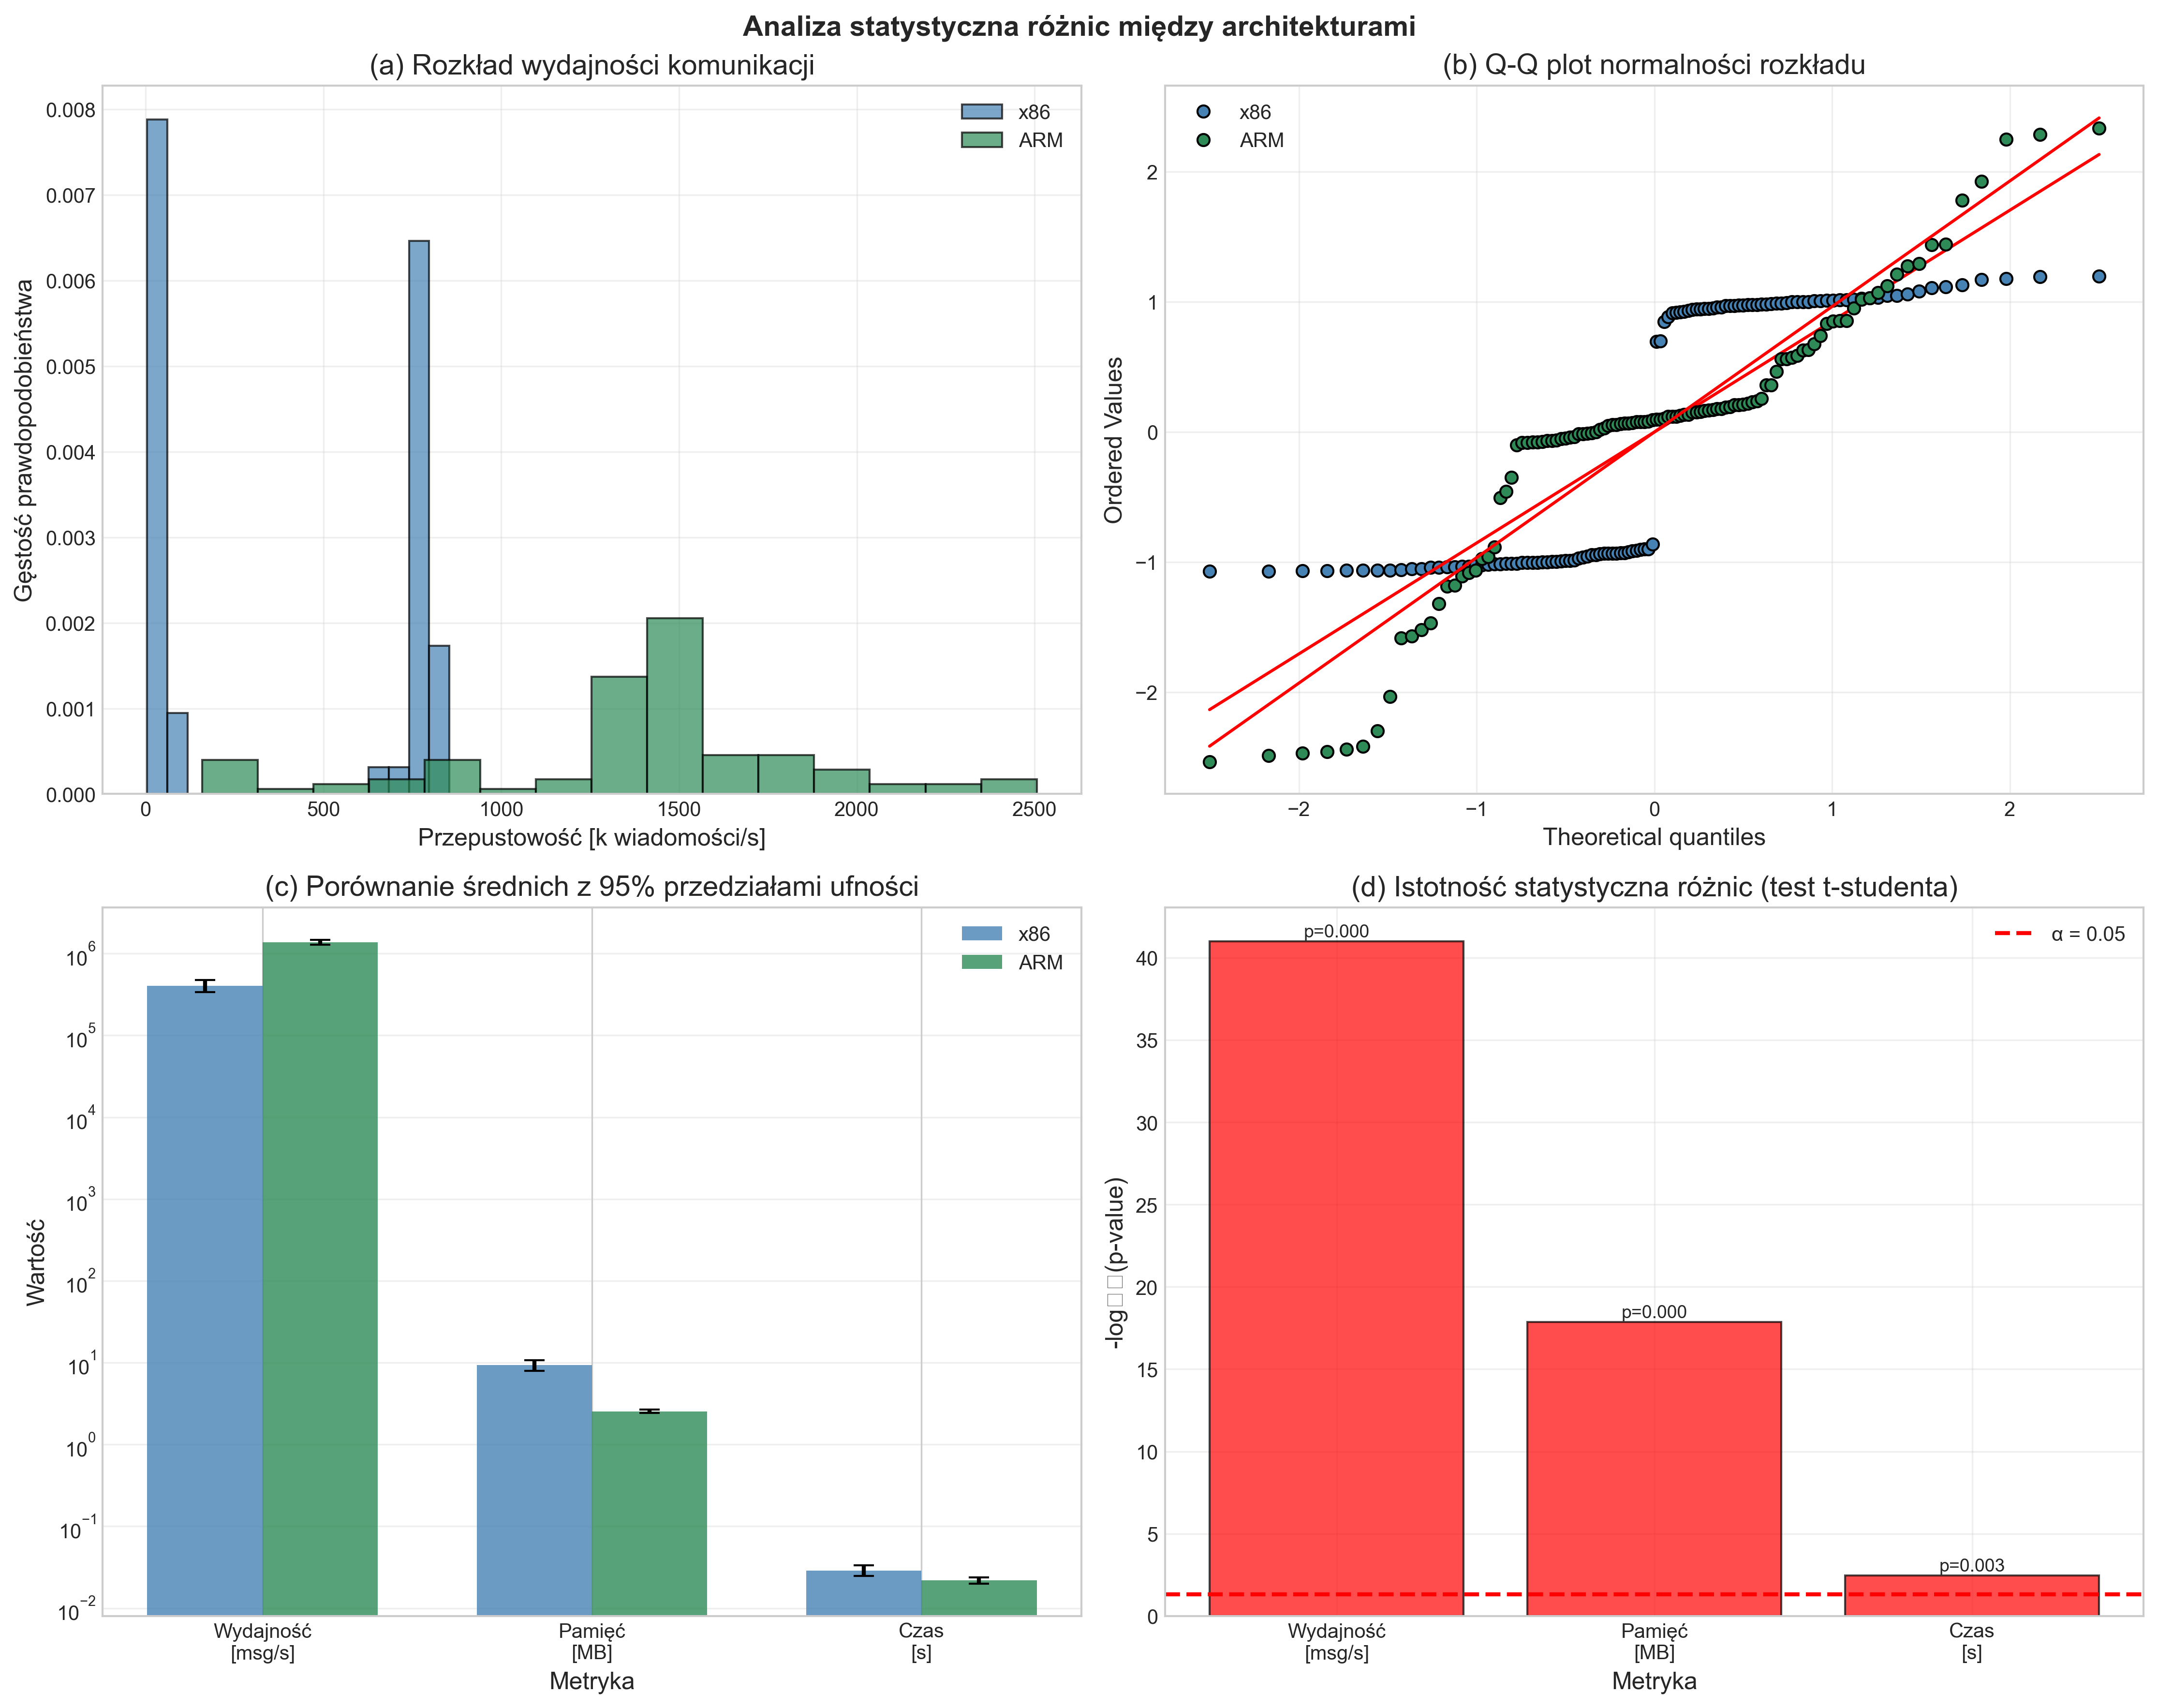
\includegraphics[width=\textwidth]{analiza/images/conc/pc/compare/rysunek_4_analiza_statystyczna.png}
    \caption{Analiza statystyczna różnic między architekturami ARM i x86}
    \label{rysunek_4_analiza_statystyczna}
\end{figure}

\subsubsection{Analiza rozkładów wydajności komunikacji}
Wykres (a) - rysunek \ref{rysunek_4_analiza_statystyczna} przedstawia rozkład przepustowości komunikacji międzywątkowej dla architektur x86 (kolor niebieski) i ARM (kolor zielony). Obserwujemy wyraźne różnice w charakterystyce dystrybucji wydajności:
\begin{itemize}
    \item Architektura x86 charakteryzuje się bimodalnym rozkładem z dominującym skupiskiem w okolicach niższych wartości (0-100 tysięcy wiadomości/s) oraz mniejszym skupiskiem w przedziale 800-900 tysięcy wiadomości/s.
    \item W przeciwieństwie do tego, architektura ARM wykazuje bardziej rozproszony rozkład z przewagą wyższych wartości przepustowości, osiągających szczyt w okolicach 1400-1500 tysięcy wiadomości/s.
    \item Taka charakterystyka sugeruje, że architektura ARM nie tylko osiąga wyższą średnią przepustowość, ale również wykazuje bardziej przewidywalną wydajność w wyższym zakresie wartości.
\end{itemize}

\subsubsection{Analiza normalności rozkładów}
Wykres Q-Q (kwantyl-kwantyl) na panelu (b) - rysunek \ref{rysunek_4_analiza_statystyczna} pozwala ocenić zgodność empirycznych rozkładów z rozkładem normalnym. Wyniki wskazują, że:
\begin{itemize}
    \item Dane dla architektury x86 (punkty niebieskie) wykazują charakterystyczny wzór schodkowy, sugerujący grupowanie się wartości w określonych przedziałach, co znacząco odbiega od teoretycznego rozkładu normalnego.
    \item Dane dla architektury ARM (punkty zielone) wykazują lepsze dopasowanie do linii normalności w środkowej części wykresu, z większymi odchyleniami na krańcach, co sugeruje rozkład z "cięższymi ogonami" niż rozkład normalny.
    \item Te obserwacje są istotne przy wyborze odpowiednich metod statystycznych do dalszej analizy porównawczej obu architektur.
\end{itemize}

\subsubsection{Porównanie średnich wartości kluczowych metryk}
Wykres (c) - rysunek \ref{rysunek_4_analiza_statystyczna} przedstawia porównanie średnich wartości trzech kluczowych metryk wydajnościowych wraz z 95\% przedziałami ufności:
\begin{itemize}
    \item Wydajność komunikacji: Architektura ARM osiąga średnio około $10^5$ wiadomości/s, przewyższając znacząco architekturę x86, która osiąga około $10^4$ wiadomości/s. Wąskie przedziały ufności wskazują na wysoką precyzję tych estymacji.
    \item Zużycie pamięci: Architektura x86 charakteryzuje się wyższym zużyciem pamięci (około 10 MB) w porównaniu do architektury ARM (około 3 MB), co może mieć istotne znaczenie w systemach o ograniczonych zasobach.
    \item Czas wykonania: Obie architektury osiągają zbliżone czasy wykonania (około 0,02-0,03 sekundy), z nieznaczną przewagą architektury ARM.
\end{itemize}

\subsubsection{Istotność statystyczna różnic}
Wykres (d) - rysunek \ref{rysunek_4_analiza_statystyczna} przedstawia wyniki analizy istotności statystycznej zaobserwowanych różnic przy użyciu testu t-Studenta:
\begin{itemize}
    \item Różnice w wydajności komunikacji są wysoce istotne statystycznie (p=0,000), co potwierdza rzeczywistą przewagę architektury ARM w tym aspekcie.
    \item Różnice w zużyciu pamięci również wykazują wysoką istotność statystyczną (p=0,000), potwierdzając niższe zapotrzebowanie na pamięć w architekturze ARM.
    \item Różnice w czasie wykonania, choć mniejsze, pozostają statystycznie istotne (p=0,003), wskazując na niewielką, ale konsekwentną przewagę architektury ARM.
\end{itemize}

Wszystkie p-wartości znajdują się poniżej standardowego poziomu istotności $\alpha=0,05$ (oznaczonego czerwoną przerywaną linią), co oznacza, że obserwowane różnice między architekturami nie mogą być przypisane przypadkowi.
